\documentclass{report}

\input{preamble}
\input{macros}
\input{letterfonts}
\usepackage[utf8]{inputenc}
\usepackage[T1]{fontenc}

\usepackage{chemfig}
\usepackage{multicol}
\usepackage{booktabs}
\usepackage{siunitx}
\usepackage{cancel}
\usepackage{adjustbox}
\usepackage{pdflscape}
\usepackage[backend=biber, style=apa]{biblatex}
\usepackage{caption}
\usepackage[spanish]{babel}
\usepackage{lmodern}
\usepackage{multirow}
\usepackage{tikz}
\usetikzlibrary{arrows.meta, positioning, calc, decorations.pathreplacing, babel, shapes.geometric}
\usepackage{amsmath}
\usepackage{minted}
\usepackage{csquotes}
\usepackage{subcaption}
\usepackage{float}
\addto\captionsspanish{
  \renewcommand{\contentsname}{Índice}
}

\usepackage{fancyhdr}
\pagestyle{fancy}
\fancyhf{}
\fancyhead[R]{Pérez Hita, Christian (christianperez@correo.ugr.es)}
\fancyfoot[C]{\thepage}

\title{\Huge{ 
\includegraphics[width=0.4\textwidth]{escudo.png}\\[2cm] Prácticas de Scilab}\\Reactor Discontinuo Mezcla Perfecta (RDMP)}
\author{\huge{Christian Pérez Hita}}
\date{}

\begin{document}
\spanishdeactivate{.<>}
\maketitle

\qs{RDMP-1}{En un reactor discontinuo mezcla perfecta isotermo, se lleva a cabo la siguiente reacción química:
	A $\rightarrow$ B \\
	Constante de velocidad = 0.5 h$^{-1}$
	El reactor se pone en marcha con 1 mol/L de A.
	\begin{enumerate}[label=\bfseries\tiny\protect\circled{\small\Alph*}]
		\item Obtener la dinámica durante 5 h de reacción, es decir, la evolución temporal de las concentraciones de A y B, así como de la conversión
	\end{enumerate}}
\solve{}
\begin{minted}[fontsize=\small, linenos]{scilab}
clear; clc; 
// RDMP-1.sce
// A => B

// Isotermo     

//! acumulacion v*ca 

//* SISTEMA DE ECUACIONES DIFERENCIALES
function dxdt = f(t,x)
    // Variables diferenciales
    CA = x(1)
    CB = x(2)
    // Velocidad de reacción
    r = k*CA
    // Balance de materia para A
    // d(V*CA)dt = -r*V
    dCAdt = -r
    // Balance de materia para B
    // d(V*CB)dt = r*V
    dCBdt =  r
    // Derivadas
    dxdt(1) = dCAdt
    dxdt(2) = dCBdt
endfunction

// CONSTANTES
k = 0.5; // h-1

// CONDICIONES INICIALES
CAini = 1; CBini = 0; // mol/L
xini = [CAini;CBini];

// TIEMPO
tfin = 5; dt = 0.01; t = 0:dt:tfin; // h-1

// RESOLVER
x = ode(xini,0,t,f);
CA = x(1,:); CAfin = CA($)
CB = x(2,:); CBfin = CB($)

XA = 1 - CA/CAini; XAfin = XA($)

// GRÁFICAS
scf(1); clf(1);
plot(t,CA,t,CB);
xgrid; xlabel('t'); legend('CA','CB',-2,%f);

scf(2); clf(2); 
plot(t,XA,'m-');
xgrid; xlabel('t'); legend('XA',-2,%f);

disp('Concentracion final de A: '+string(CAfin)+' mol/L');
disp('Concentracion final de B: '+string(CBfin)+' mol/L');
disp('Conversión final de A: '+string(XAfin)+' mol/L');
\end{minted}
\nt{En resultado se muestra lo que aparece en pantalla al ejecutar el código:}
\Res{
	\begin{array}{l}
		\text{Concentración final de A: 0.082085 mol/L} \\
		\text{Concentración final de B: 0.917915 mol/L} \\
		\text{Conversión final de A: 0.917915 mol/L}
	\end{array}
}
\begin{figure}[H]
	% Centramos todo el bloque de la figura
	\makebox[\textwidth][c]{
		\begin{subfigure}[b]{0.6\textwidth} % Aumentamos el contenedor de la subfigura al 60%
			\centering
			% La imagen ocupa el 100% de SU contenedor (que ya es grande)
			
\includegraphics[width=\linewidth]{RDMP_1.1.png}
			\caption{Concentraciones de A y B}
			\label{fig:RDMP-1_1}
		\end{subfigure}

		\hspace{-0.05\textwidth} % Espacio negativo para acercarlas un poco si se separan mucho

		\begin{subfigure}[b]{0.6\textwidth} % Segunda subfigura también al 60%
			\centering
			
\includegraphics[width=\linewidth]{RDMP_1.2.png}
			\caption{Conversión de A}
			\label{fig:RDMP-1_2}
		\end{subfigure}
	}

	% Leyenda principal para todo el conjunto
	\vspace{1ex} % Un pequeño espacio vertical antes de la leyenda
	\caption{Evolución temporal del reactor por lotes}
	\label{fig:RDMP-agrupado}
\end{figure}
\qs{RDMP-2}{La reacción química
	A $\rightarrow$ B

	Factor preexponencial = 4.15E5 s$^{-1}$\\
	Energía de activación = 11200 cal/mol\\
	Entalpía de reacción = -50400  cal/mol

	Se lleva a cabo en un reactor discontinuo mezcla perfecta adiabático que se pone en marcha con 0.5 mol/L de A a 285 K.
	Considerando para la mezcla reaccionante una capacidad calorífica de 0.9 cal/(g*K) y una densidad de 1070 g/L:
	\begin{enumerate}[label=\bfseries\tiny\protect\circled{\small\Alph*}]
		\item Obtener la dinámica del proceso
		\item Determinar la temperatura cuando se alcanza el 90$\%$ de conversión
	\end{enumerate}}
\newpage
\solve{}
\begin{minted}[fontsize=\small, linenos]{scilab}
//  d(V*CA)dt = -r*V consume a por eso es -r y el reacto de a es r lo consumido *v
//  v es constante por lo que puede salir de la derivada
//  dCAdt = -r  
//  Variables diferenciales como ya tenemos CA en una ec definida la ponemos como constante 
//  d(V*RHO*CP*T)dt  //<····(m·cp·t)//= -H*r*V ; el signo menos de la entalpia es por que al ser 
//  exotermica por convenio la h es negativa y como tiene que aumentar 
//  la temperatura es necesario para -·-=*  // dTdt  = -H*r/(RHO*CP)   

// si la reaccion es irreversible no se suele poner los balances de materia del producto 
// se puede hacer aunque no sea necesario ya que la potencia de calculo no la complica

// en los ejercicios nunca vamos  a tener que realizar cambios de unidades pero si poner las unidades
// constante que buscar siempre la r es decir tenerlas tabuladas

// el tiempo no nos lo da el ejercicio ponemos un numero provisional de prueba y error

// xgrid; xlabel('t'); legend('CA',-2,%f);
// xgrid; xlabel('t'); legend('XA',-2,%f);
// plot(t,T,'r-',tXAobj,TXAobj,'ro');
// xgrid; xlabel('t'); legend('T',-2,%f);// el ,-2 es la posicion arriba izquiera fuera
// el -3 es abajo izquierda fuera del grafico , el %f es para eliminar la caja de la leyenda


clear; clc;
// RDMP-2.sce
// A => B
// Adiabático

// SISTEMA DE ECUACIONES DIFERENCIALES
function dxdt = f(t, x)
    CA = x(1);
    T  = x(2);
    
    // Ecuación de Arrhenius
    k = k0 * exp(-E / (R * T));
    
    // Velocidad de reacción
    r = k * CA;
    
    // Balance de materia para A
    dCAdt = -r;
    
    // Balance de energía
    dTdt = -H * r / (RHO * CP);
    
    // Retornar como columna
    dxdt = [dCAdt; dTdt]; 
endfunction

// CONSTANTES
CP = 0.9; // cal/(g*K)
RHO = 1070; // g/L
H = -50400; // cal/mol  //* Reacción exotérmica ya que la entalpia de reaccion tiene signo negativo
k0 = 4.15E5; // s-1
E = 11200; // cal/mol
R = 1.987; // cal/(mol*K)



// CONDICIONES INICIALES
CAini = 0.5; // mol/L
Tini = 285; // K
xini = [CAini; Tini];

// TIEMPO INICIAL
tfin = 50; dt = 1;
XAobj = 0.90; // Conversión objetivo
XAalcanzado = 0; // Variable para comprobar si se alcanza XAobj
tfinal_max = 10000; // Tiempo máximo permitido
t = 0:dt:tfin; 

// SOLVER
while (XAalcanzado < XAobj & tfin < tfinal_max)
    x = ode(xini, 0, t, f);
    
    // Extraer valores de concentración y temperatura
    CA = x(1, :);
    T = x(2, :);
    
    // Calcular conversión
    XA = 1 - CA / CAini;
    
    // Revisar si se alcanzó el valor objetivo
    if max(XA) >= XAobj then
        XAalcanzado = max(XA);
        break; // Termina el bucle si se alcanza la conversión objetivo
    else
        // Aumentar el tiempo de simulación si no se alcanza XAobj
        tfin = tfin + 50;
        t = 0:dt:tfin;
    end
end

// Encontrar el tiempo en que se alcanza XAobj
indexXAobj = find(XA >= XAobj, 1);
if indexXAobj <> [] then
    tXAobj = t(indexXAobj);
    TXAobj = T(indexXAobj);
else
    tXAobj = NaN;
    TXAobj = NaN;
end

// GRÁFICAS
scf(1); clf(1); 
plot(t, CA, 'b');
xgrid; xlabel('t'); legend('CA', -2, %f);

scf(2); clf(2); 
plot(t, XA, 'm-', tXAobj, XAobj, 'mo');
xgrid; xlabel('t'); legend('XA', -2, %f);

scf(3); clf(3); 
plot(t, T, 'r-', tXAobj, TXAobj, 'ro');
xgrid; xlabel('t'); legend('T', -2, %f);
disp('la conversion de A es de '+string(XAalcanzado*100)+'%');
disp('la temperatura en la que se alcanza el 90% de conversion es de '+string(TXAobj)+' K');
disp('el tiempo en el que se alcanza el 90% de conversion es de '+string(tXAobj)+' s');
disp('el tiempo maximo permitido es de '+string(tfinal_max)+' s');
\end{minted}
\Res{\begin{array}{l}
		\text{la conversion de A es de 90.551024\%}                                        \\
		\text{la temperatura en la que se alcanza el 90\% de conversion es de 308.55992 K} \\
		\text{el tiempo en el que se alcanza el 90\% de conversion es de 839 s}            \\
		\text{el tiempo maximo permitido es de 10000 s}                                    \\
	\end{array}}
% --- FIGURA INDEPENDIENTE (Imagen A) ---
\begin{figure}[H]
	\centering
	
\includegraphics[width=1\textwidth]{RDMP_2.1.png} % Ajusta el tamaño a tu gusto
	\caption{Concentración de A}
	\label{fig:RDMP-2_1}
\end{figure}

% --- FIGURA CON SUBPLOTS (Imágenes B y C) ---
\begin{figure}[H]
	\centering
	% El makebox permite que las imágenes se expandan hacia los márgenes simétricamente
	\makebox[\textwidth][c]{
		\begin{subfigure}[b]{0.6\textwidth} % Aumentado un ~10-12% respecto al original
			\centering
			
\includegraphics[width=\linewidth]{RDMP_2.2.png}
			\caption{Conversión de A}
			\label{fig:RDMP-2_2}
		\end{subfigure}

		\hspace{1em} % Pequeño espacio de separación

		\begin{subfigure}[b]{0.6\textwidth}
			\centering
			
\includegraphics[width=\linewidth]{RDMP_2.3.png}
			\caption{Temperatura}
			\label{fig:RDMP-2_3}
		\end{subfigure}
	}
	\vspace{1ex}
	\caption{Evolución de la conversión y temperatura en el reactor}
	\label{fig:RDMP-subplots}
\end{figure}
\qs{RDMP-3a}{La reacción química
	A $\rightarrow$ B

	Factor preexponencial = 2.2E4 s$^{-1}$\\
	Energía de activación = 41570  J/mol\\
	Entalpía de reacción = -5E5  J/mol

	Se lleva a cabo durante 1500 s en un reactor discontinuo mezcla perfecta de 1 m$^3$ que dispone de una camisa de 4 m$^2$ a 283 K
	con un coeficiente global de transmisión de calor de 400 J/(m2·s·K).
	Considerando para la mezcla reaccionante una densidad de 980 kg/m$^3$ y una capacidad calorífica de 4200 J/(kg·K):
	\begin{enumerate}[label=\bfseries\tiny\protect\circled{\small\Alph*}]
		\item Obtener la dinámica del proceso si el reactor se pone en marcha con 500 mol/m$^3$ de A a 283 K
		\item Localizar el instante de temperatura máxima
	\end{enumerate}}
\solve{}
\begin{minted}[fontsize=\small, linenos]{scilab}

  clear; clc; 
// RDMP-3a.sce
// A => B
// No adiabático: camisa a temperatura constante

// SISTEMA DE ECUACIONES DIFERENCIALES
function dxdt = f(t,x)
    // Variables diferenciales
    CA = x(1)
    T  = x(2)
    // Ecuación de Arrhenius
    k = k0*exp(-E/(R*T))
    // Velocidad de reacción
    r = k*CA
    // Calor transferido del reactor a la camisa
    Q = U*A*(T-TJ)
    // Balance de materia para A
    // d(V*CA)dt = -r*V
    dCAdt = -r                             
    // Balance de energía no hay entrada ni salida solo generacion 
    //consideracion camisas en reactores y serpentines refrigeran por ello el signo -
    // y ponemos -Q que hay que calcularlo (linea 16)
    // d(V*RHO*CP*T)dt = -H*r*V - Q
    dTdt = -H*r/(RHO*CP) -  Q/(V*RHO*CP)   
    // Derivadas
    dxdt(1) = dCAdt
    dxdt(2) = dTdt
endfunction

// CONSTANTES
V = 1; // m3
RHO = 980; // kg/m3
CP = 4200; // J/(kg*K)
U = 400; // J/(m2*s*K)
A = 4; // m2
TJ = 283; // K
H = -5E5; // J/mol
k0 = 2.2E4; // s-1
E = 41570; // J/mol
R = 8.314; // J/(mol*K)

// CONDICIONES INICIALES
CAini = 500; // mol/m3
Tini = 283; // K
xini = [CAini; Tini];

// TIEMPO
tfin = 1500; dt = 1; t = 0:dt:tfin; // s

// RESOLVER
x = ode(xini,0,t,f);
CA = x(1,:); CAfin = CA($)
T = x(2,:); Tfin = T($)

[Tmax,indexTmax] = max(T)
tTmax = t(indexTmax)
disp(' La temperatura maxima es: '+string(Tmax)+' K')
disp(' El tiempo en el que se alcanza la temperatura maxima es: '+string(tTmax)+' s')

// GRÁFICAS
scf(1); clf(1); 
plot(t,CA);
xgrid; xlabel('t'); legend('CA',-2,%f);

scf(2); clf(2); 
plot(t,T,'r-',tTmax,Tmax,'ro');
xgrid; xlabel('t'); legend('T',-2,%f);
\end{minted}
\Res{
	\begin{array}{l}
		\text{La temperatura maxima es: 329.26838 K} \\
		\text{El tiempo en el que se alcanza la temperatura maxima es: 1191 s}
	\end{array}
}

\begin{figure}[H]
	\centering
	% El makebox permite que las imágenes se expandan hacia los márgenes simétricamente
	\makebox[\textwidth][c]{
		\begin{subfigure}[b]{0.6\textwidth} % Aumentado un ~10-12% respecto al original
			\centering
			
\includegraphics[width=\linewidth]{RDMP_3.1A.png}
			\caption{Conversión de A}
			\label{fig:RDMP-3.1A}
		\end{subfigure}

		\hspace{1em} % Pequeño espacio de separación

		\begin{subfigure}[b]{0.6\textwidth}
			\centering
			
\includegraphics[width=\linewidth]{RDMP_3.2A.png}
			\caption{Temperatura}
			\label{fig:RDMP-3.2}
		\end{subfigure}
	}
	\vspace{1ex}
	\caption{Evolución de la conversión y temperatura en el reactor}
	\label{fig:RDMP-3A-subplots}
\end{figure}
\qs{RDMP-3b}{La reacción química
	A $\rightarrow$ B

	Factor preexponencial = 2.2E4 s$^{-1}$\\
	Energía de activación = 41570  J/mol\\
	Entalpía de reacción = -5E5  J/mol

	se lleva a cabo durante 1500 s en un reactor discontinuo mezcla perfecta de 1 m$^3$
	que dispone de una camisa de 0.1 m$^3$ y 4 m$^2$ capaz de transmitir calor con un coeficiente global de 400 J/(m2·s·K)
	y por la que circulan 0.001 m$^3$/s de agua que entran a 283 K. Considerando para la mezcla reaccionante una densidad de 980 kg/m$^3$
	y una capacidad calorífica de 4200 J/(kg·K):
	\begin{enumerate}[label=\bfseries\tiny\protect\circled{\small\Alph*}]
		\item Obtener la dinámica del proceso si el reactor se pone en marcha con 500 mol/m$^3$ de A a 283 K
		\item Determinar el caudal de agua que debe circular por la camisa para que la temperatura del reactor no supere en ningún momento los 330 K
	\end{enumerate}}
\begin{minted}[fontsize= \small, linenos]{scilab}
  clear; clc; 
// RDMP-3b.sce
// A => B
// No adiabático: camisa a temperatura variable

// SISTEMA DE ECUACIONES DIFERENCIALES
function dxdt = f(t,x)
    // Variables diferenciales
    CA = x(1)
    T  = x(2)
    TJ = x(3)
    // Ecuación de Arrhenius
    k  = k0*exp(-E/(R*T))
    // Velocidad de reacción
    r  = k*CA
    // Calor transferido del reactor a la camisa
    Q  = U*A*(T-TJ)
    // Balance de materia para A (no hace falta el balance para b)
    // d(V*CA)dt = -r*V
    dCAdt = -r  
    // Balance de energía en el reactor
    // d(V*RHO*CP*T)dt = -H*r*V - Q
    dTdt  = -H*r/(RHO*CP)  - Q/(V*RHO*CP)
    // Balance de energía en la camisa
    // d(VJ*RHOJ*CPJ*TJ)dt =  FJ*RHOJ*CPJ*TJ0 - FJ*RHOJ*CPJ*TJ + Q
    //hay 2 terminos sale la constante por lo que queda la derivada de TJ que es x(3)
    dTJdt = FJ*(TJ0-TJ)/VJ + Q/(VJ*RHOJ*CPJ)  
    // Derivadas
    dxdt(1) = dCAdt
    dxdt(2) = dTdt
    dxdt(3) = dTJdt
endfunction

// CONSTANTES
V = 1; // m3
RHO = 980; // kg/m3
CP = 4200; // J/(kg*K)
U = 400; // J/(m2*s*K)
A = 4; // m2
VJ = 0.1; // m3
FJ = 6.15E-3; //m3/s
TJ0 = 283 // // K
RHOJ = 1000; // kg/m3
CPJ = 4180; //J/(kg*K)
H = -5E5; // J/mol
k0 = 2.2E4; // s-1
E = 41570; // J/mol
R = 8.314; // J/(mol*K)

// CONDICIONES INICIALES
CAini = 500; // mol/m3
Tini = 283; // K
TJini = 283; // K
//el valor inicial de la camisa no nos lo dice asi que supones 283
//asumimos que inicialmente el reactor y la camisa estan a la misma T
xini = [CAini; Tini; TJini];

// TIEMPO
tfin = 1500; dt = 1; t = 0:dt:tfin; // s

// RESOLVER
x = ode(xini,0,t,f);
CA = x(1,:); CAfin = CA($);
T = x(2,:); Tfin = T($);
TJ = x(3,:); TJfin = TJ($);
disp("La concentracion final de A es: "+ string(CAfin) + " mol/m3")
disp("La temperatura final del reactor es: "+ string(Tfin) + " K")
disp("La temperatura final de la camisa es: "+ string(TJfin) + " K")
[Tmax,indexTmax] = max(T);
tTmax = t(indexTmax);
disp("La temperatura maxima es: "+ string(Tmax) + " K" + " y se alcanza en el instante " + string(tTmax) + " s")
// GRÁFICAS
scf(1); clf(1);
plot(t,CA);
xgrid; xlabel('t'); legend('CA',-2,%f);

scf(2); clf(2);
plot(t,T,'r-',t,TJ,'r:',tTmax,Tmax,'ro');
xgrid; xlabel('t'); legend('T','TJ',-2,%f);

scf(3); 
plot(FJ,Tmax,'ro');
xgrid; xlabel('FJ'); ylabel('Tmax');

//para saber el caudal de tj lo cambiamos pot tanteo por intuicion ya que queremos que tmax sea la 
//t final o haciendo un bucle probar en casa bucle para calcular el caudal necesario
//que mantenga el reactor por debajo de 330º
//if tmax> T  then  Fj=FJi+0.01meter tambien un epsilon <E2 como criterio de parada /break
//y un numero maximo de iteraciones n  entre la linea 33 y 69 
\end{minted}
\begin{figure}[h!]
	\centering
	\begin{subfigure}[b]{0.48\textwidth}
		
\includegraphics[width=\textwidth]{RDMP_3.1BREAL.png}
		\caption{Conversión de A vs t}
		\label{fig:RDMP-3.1BREAL}
	\end{subfigure}
	\hfill
	\begin{subfigure}[b]{0.48\textwidth}
		
\includegraphics[width=\textwidth]{RDMP_3.2BREAL.png}
		\caption{Temperaturas vs t}
		\label{fig:RDMP-3.2BREAL}
	\end{subfigure}
\end{figure}
\begin{figure}[h!]
	\centering
	
\includegraphics[width=0.65\textwidth]{RDMP_3.3BREAL.png}
	\caption{Temperatura}
	\label{fig:RDMP-3.3BREAL}
\end{figure}
\Res{
	\begin{array}{l}
		\text{La concentracion final de A es: } 4.4895026 \text{ mol/m}^3 \\
		\text{La temperatura final del reactor es: } 327.25683 \text{ K}  \\
		\text{La temperatura final de la camisa es: } 285.605 \text{ K}   \\
		\text{La temperatura maxima es: } 329.99939 \text{ K y se alcanza en el instante } 1192 \text{ s}
	\end{array}
}
\newpage
\qs{RDMP-3c}{La reacción química
	A $\rightarrow$ B

	Factor preexponencial = 2.2E4 s$^{-1}$\\
	Energía de activación = 41570  J/mol\\
	Entalpía de reacción = -5E5  J/mol

	se lleva a cabo durante 1500 s en un reactor discontinuo mezcla perfecta de 1 m$^3$
	que dispone de un serpentín de 13 m de longitud y 0.1 m de diámetro capaz de transmitir calor con un coeficiente
	global de 400 J/(m2·s·K) y por el que circulan 0.001 m$^3$/s de agua que entran a 283 K. Considerando para la mezcla
	reaccionante una densidad de 980 kg/m$^3$ y una capacidad calorífica de 4200 J/(kg·K):
	\begin{enumerate}[label=\bfseries\scriptsize\protect\circled{\footnotesize\Alph*}]
		\item Obtener la dinámica del proceso si el reactor se pone en marcha con 500 mol/m$^3$ de A a 283 K
	\end{enumerate}}
\begin{minted}[fontsize=\small, linenos]{scilab}
clear; clc; 
// RDMP-3c.sce
// A => B
// No adiabático: serpentín
//matiz ejercicio dificil 
// SECTORES
N = 10; // divisiones del serpentín

// SISTEMA DE ECUACIONES DIFERENCIALES
function dxdt = f(t,x)
    // Variables diferenciales
    Ts = x(1:N)
    CA = x(N+1)
    T  = x(N+2)
    // Calor transferido del reactor al serpentín
    i = 1:N; Q(i) = U*As*(T-Ts(i));
    // Balance de energía en el serpentín
    // d(Vs*RHOs*CPs*Ts(i))dt =  Fs*RHOs*CPs*Ts(i-1) - Fs*RHOs*CPs*Ts(i) + Q(i)
    // Sector 1 como no puede ser i-1  tiene su propio balance abajo
    dTsdt(1) = Fs*(Ts0-Ts(1))/Vs + Q(1)/(Vs*RHOs*CPs)
    // Resto de sectores
    i = 2:N; dTsdt(i) = Fs*(Ts(i-1)-Ts(i))/Vs + Q(i)/(Vs*RHOs*CPs)
    // Ecuación de Arrhenius
    k = k0*exp(-E/(R*T))
    // Velocidad de reacción
    r = k*CA
    // Balance de materia para A
    // d(V*CA)dt = -r*V
    dCAdt = -r  
    // Balance de energía en el reactor
    // d(V*RHO*CP*T)dt = -H*r*V - Q
    dTdt  = -H*r/(RHO*CP) - sum(Q)/(V*RHO*CP)  
    // Derivadas
    dxdt(1:N) = dTsdt
    dxdt(N+1) = dCAdt
    dxdt(N+2) = dTdt
endfunction

// CONSTANTES
V = 1; // m3
RHO = 980; // kg/m3
CP = 4200; //J/(kg*K)

U = 400; // J/(m2*s*K)
Ds = 0.1; // m
Lstot = 13; // m
Vstot = %pi/4*Ds^2*Lstot // m3 (volumen de sector total)
Astot = %pi*Ds*Lstot  // m2
Vs = Vstot/N;  // m3 (volumen de sector)
As = Astot/N;  // m2 (area de sector)
Fs = 1E-3; //m3/s (flujo serpentin)
Ts0 = 283; // K
RHOs = 1000; // kg/m3
CPs = 4180; //J/(kg*K)

H = -5E5; // J/mol
k0 = 2.2E4; // s-1
E = 41570; // J/mol
R = 8.314; // J/(mol*K)

// CONDICIONES INICIALES
i = 1:N; Tsini(i) = 283; // K iniciando todos los sectores a t inciial 
CAini = 500; // mol/m3
Tini = 283; // K
xini = [Tsini; CAini; Tini];

// TIEMPO
tfin = 1500; dt = 1; t = 0:dt:tfin; // s

// RESOLVER
x = ode(xini,0,t,f);
disp(size(x))
Ts = x(1:N,:); Tsfin = Ts(:,$);
CA = x(N+1,:); CAfin = CA($);
T  = x(N+2,:); Tfin = T($);

[Tmax,indexTmax] = max(T);
tTmax = t(indexTmax);

// GRÁFICAS
scf(1); clf(1);
plot(t,CA);
xgrid; xlabel('t'); legend('CA',-2,%f);

scf(2); clf(2);
plot(t,T,'r-',t,Ts,'r:',tTmax,Tmax,'ro');
xgrid; xlabel('t'); legend('T','Ts',-2,%f);

scf(3); clf(3);
plot(Tsini,'ro-');      // t=0
plot(Ts(:,$/2),'ro-');  // t=tfin/2
plot(Tsfin,'ro-');      // t=tfin
xgrid; xlabel('Sector'); ylabel('Ts');

disp("El volumen del serpentín es:" + string(Vstot) + "m3")
disp("El area del serpentín es:" + string(Astot) + "m2")
disp("el volumen del sector es:" + string(Vs) + "m3")
disp("el area del sector es:" + string(As) + "m2")
disp("la temperatura de salida de los sectores del serpetin son:")
for i = 1:N+1 
    if i < N+1 then 
        disp("la temperatura de salida del sector " + string(i) + " es:" + string(Tsfin(i)) + "K")
    else 
        disp("la temperatura de salida del reactor es:" + string(Tfin) + "K")
    end
end
disp("la temperatura maxima en el reactor es:" + string(Tmax) + "K" +" que se da a los " + string(indexTmax) + "s del inicio del proceso")
disp("el tiempo en el que se alcanza la temperatura maxima es:" + string(tTmax) + "s")

// Si quiero que el refrigerante sea el necesario para que Tmax = Tfin
// ITERACIÓN SOBRE Fs
tol = 1e-2;        // tolerancia (K)
max_iter = 1000;    // seguridad
iter = 0;

while iter < max_iter
    
    // Resolver sistema
    x = ode(xini,0,t,f);
    
    Ts = x(1:N,:);
    CA = x(N+1,:);
    T  = x(N+2,:);
    
    Tfin = T($);
    Tmax = max(T);
    
    // Condición de convergencia
    if abs(Tmax - Tfin) < tol then
        break
    end
    
    // Ajuste de Fs
    if Tmax > Tfin then
        // sobreenfriando → demasiado refrigerante
        Fs = Fs - Fs/70;
    else
        // falta refrigeración
        Fs = Fs + Fs/70;
    end
    
    iter = iter + 1;
end

disp("Fs óptimo aproximado: " + string(Fs))
disp("Iteraciones: " + string(iter))
disp("Tmax = " + string(Tmax) + "K" + " Tfin = " + string(Tfin) + "K" + " Diferencia = " + string(abs(Tmax - Tfin)) + "K")
\end{minted}
\begin{figure}[h!]
	\centering
	\begin{subfigure}[b]{0.48\textwidth}
		
\includegraphics[width=\textwidth]{RDMP_3.1CREAL.png}
		\caption{Conversión de A vs t}
		\label{fig:RDMP-3.1CREAL}
	\end{subfigure}
	\hfill
	\begin{subfigure}[b]{0.48\textwidth}
		
\includegraphics[width=\textwidth]{RDMP_3.2CREAL.png}
		\caption{Temperaturas vs t}
		\label{fig:RDMP-3.2CREAL}
	\end{subfigure}
	\label{fig:RDMP-3CREAL}
\end{figure}
\begin{figure}[h!]
	\centering
	
\includegraphics[width=0.5\textwidth]{RDMP_3.3CREAL.png}
	\caption{Temperatura}
	\label{fig:RDMP-3.3CREAL}
\end{figure}
\Res{
	\begin{array}{l}
		12.   1501.                                                                                                  \\
		\text{El volumen del serpentín es:}0.1021018\text{m}3                                                        \\
		\text{El area del serpentín es:}4.0840704\text{m}2                                                           \\
		\text{el volumen del sector es:}0.0102102\text{m}3                                                           \\
		\text{el area del sector es:}0.408407\text{m}2                                                               \\
		\text{la temperatura de salida de los sectores del serpetin son:}                                            \\
		\text{la temperatura de salida del sector 1 es:}284.72647\text{K}                                            \\
		\text{la temperatura de salida del sector 2 es:}286.39235\text{K}                                            \\
		\text{la temperatura de salida del sector 3 es:}287.99969\text{K}                                            \\
		\text{la temperatura de salida del sector 4 es:}289.5505\text{K}                                             \\
		\text{la temperatura de salida del sector 5 es:}291.04671\text{K}                                            \\
		\text{la temperatura de salida del sector 6 es:}292.49017\text{K}                                            \\
		\text{la temperatura de salida del sector 7 es:}293.88269\text{K}                                            \\
		\text{la temperatura de salida del sector 8 es:}295.226\text{K}                                              \\
		\text{la temperatura de salida del sector 9 es:}296.52177\text{K}                                            \\
		\text{la temperatura de salida del sector 10 es:}297.77162\text{K}                                           \\
		\text{la temperatura de salida del reactor es:}328.78124\text{K}                                             \\
		\text{la temperatura maxima en el reactor es:}331.28838\text{K que se da a los 1199s del inicio del proceso} \\
		\text{el tiempo en el que se alcanza la temperatura maxima es:}1198\text{s}                                  \\
		\text{Fs óptimo aproximado: }5.637\text{D-10}                                                                \\
		\text{Iteraciones: }1000                                                                                     \\
		\text{Tmax = }338.2411\text{K Tfin = }338.22913\text{K Diferencia = }0.0119664\text{K}                       \\
	\end{array}
}
\qs{RDMP-4}{El equilibrio químico

	A + B  $\rightleftarrows$  C

	Factor preexponencial de Arrhenius = 1.75E8 L/(mol·h)\\
	Factor preexponencial de Van't Hoff = 8.25E-22 L/mol\\
	Energía de activación = 62350 J/mol\\
	Entalpía de reacción = -136400 J/mol

	se pone en marcha en un reactor discontinuo mezcla perfecta adiabático con 1 moL/L de A y 2 mol/L de B a 300 K.
	Considerando para la mezcla reaccionante una densidad de 1150 g/L y una capacidad calorífica de 3.8 J/(g·K):
	\begin{enumerate}[label=\bfseries\scriptsize\protect\circled{\footnotesize\Alph*}]
		\item Obtener la dinámica del proceso
		\item Determinar cuándo se alcanza el equilibrio, definido por una derivada absoluta de la temperatura inferior a 1E-3 K/h
		\item Estudiar la influencia de la temperatura inicial en la conversión de equilibrio y en el tiempo necesario para alcanzar el 50$\%$ de conversión
	\end{enumerate}}
\begin{minted}[fontsize=\small, linenos]{scilab}
clear; clc; 
// RDMP-4.sce
// 2 A <=> B
// Isotermo

// SISTEMA DE ECUACIONES DIFERENCIALES
function dxdt = f(t,x)
    // Variables diferenciales
    CA = x(1)
    CB = x(2)
    // Velocidad de reacción
    // r = rd - ri = kd*CA^2 - ki*CB = kd*CA^2 - kd*CB/Keq
    r = kd*(CA^2 - CB/Keq)
    // Balance de materia para A
    // d(V*CA)dt = -r*V
    dCAdt = -r 
    // Balance de materia para B
    // d(V*CB)dt = r/2*V
    dCBdt = r/2
    // Derivadas
    dxdt(1) = dCAdt
    dxdt(2) = dCBdt
endfunction

// CONSTANTES
T = 420; // K
kd0 = 1.4E12; // L/(mol*h)
E = 105000; // J/mol
Keq0 = 6.9E8; // L/mol
H = 63000; // J/mol
R = 8.314; // J/(mol*K)
kd = kd0*exp(-E/(R*T))   // Ecuación de Arrhenius
Keq = Keq0*exp(-H/(R*T)) // Ecuación de Van't Hoff

// CONDICIONES INICIALES
CAini = 5; CBini = 0; // mol/L
xini = [CAini; CBini];

// TIEMPO
tfin = 100; dt = 0.1; t = 0:dt:tfin; // h

// RESOLVER
x = ode(xini,0,t,f);
CA = x(1,:); CAfin = CA($);
CB = x(2,:); CBfin = CB($);
disp('Concentracion final de A: '+string(CAfin)+' mol/L');
disp('Concentracion final de B: '+string(CBfin)+' mol/L');

dCAdt = diff(CA)/dt; dCBdt = diff(CB)/dt; 
dCAdteq = 1E-5; dCBdteq = 1E-5; // mol/(L*h)
indexCAeq = find(abs(dCAdt)<dCAdteq,1); indexCBeq = find(abs(dCBdt)<dCBdteq,1);
tCAeq = t(indexCAeq), tCBeq = t(indexCBeq);
CAeq = CA(indexCAeq), CBeq = CB(indexCBeq);
disp('Tiempo de equilibrio para CA: '+string(tCAeq)+' h');
disp('Concentracion de equilibrio para CA: '+string(CAeq)+' mol/L');
disp('Tiempo de equilibrio para CB: '+string(tCBeq)+' h');
disp('Concentracion de equilibrio para CB: '+string(CBeq)+' mol/L');
teq = max(tCAeq,tCBeq);
disp('Tiempo de equilibrio: '+string(teq)+' h');

indexCACB = find(CA<CB,1);
tCACB = t(indexCACB);
CACB = CA(indexCACB);
disp('Tiempo en que CA = CB: '+string(tCACB)+' h');

// GRÁFICAS
scf(1); clf(1); 
plot(t,CA,t,CB);
plot(tCAeq,CAeq,'b.',tCBeq,CBeq,'g.');
plot(tCACB,CACB,'bo');
xgrid; xlabel('t'); legend('CA','CB',-2,%f);

scf(2); clf(2); 
plot(t(1:$-1),abs(dCAdt),t(1:$-1),abs(dCBdt));
plot(tCAeq,dCAdteq,'b.',tCBeq,dCBdteq,'g.'); 
xgrid; xlabel('t'); legend('|dCAdt|','|dCBdt|',-2,%f);
a2 = gca; a2.log_flags = "nl";
//! gca da el control de los ejes del grafico
//! log_flags = "nl" es para que el eje y sea logaritmico
\end{minted}
\begin{figure}[h!]
	\centering
	\begin{subfigure}[b]{0.48\textwidth}
		\centering
		
\includegraphics[width=\textwidth]{RDMP_4.1.png}
		\caption{Temperaturas vs t}
		\label{fig:RDMP-4.1}
	\end{subfigure}
	\begin{subfigure}[b]{0.48\textwidth}
		\centering
		
\includegraphics[width=\textwidth]{RDMP_4.2.png}
		\caption{Temperaturas vs t}
		\label{fig:RDMP-4.2}
	\end{subfigure}
	\caption{Dinámica del proceso}
	\label{fig:RDMP-4}
\end{figure}
\Res{
	\begin{array}{l}
		\text{Concentracion final de A: }0.4738786\text{ mol/L}            \\
		\text{Concentracion final de B: }2.2630607\text{ mol/L}            \\
		\text{Tiempo de equilibrio para CA: }75.6\text{ h}                 \\
		\text{Concentracion de equilibrio para CA: }0.473956\text{ mol/L}  \\
		\text{Tiempo de equilibrio para CB: }69.9\text{ h}                 \\
		\text{Concentracion de equilibrio para CB: }2.2629811\text{ mol/L} \\
		\text{Tiempo de equilibrio: }75.6\text{ h}                         \\
		\text{Tiempo en que CA = CB: }3.4\text{ h}                         \\
	\end{array}
}
\qs{RDMP-5}{El equilibrio químico
	2A $\rightleftarrows$  B

	Factor preexponencial de Arrhenius = 1.4E12 L/(mol·h)\\
	Factor preexponencial de Van't Hoff = 6.9E8 L/mol\\
	Energía de activación = 105000 J/mol\\
	Entalpía de reacción = 63000 J/mol

	se lleva a cabo a 420 K en un reactor discontinuo mezcla perfecta con 5 moL/L iniciales de A.
	\begin{enumerate}[label=\bfseries\scriptsize\protect\circled{\footnotesize\Alph*}]
		\item Obtener la dinámica del proceso
		\item Determinar cuándo se alcanza el equilibrio, definido por unas derivadas absolutas de las concentraciones inferiores a 1E-5 mol/(L·h)
		\item Localizar el momento en el que las concentraciones de A y B se igualan
	\end{enumerate}}

\begin{minted}[fontsize=\small, linenos]{scilab}
    clear; clc; 
// RDMP-5.sce
// A + B <=> C
// Adiabático

// SISTEMA DE ECUACIONES DIFERENCIALES
function dxdt = f(t,x)
    // Variables diferenciales
    CA = x(1)
    CB = x(2)
    CC = x(3)
    T  = x(4)
    // Ecuación de Arrhenius
    kd = kd0*exp(-E/(R*T))
    // Ecuación de Van't Hoff
    Keq = Keq0*exp(-H/(R*T))
    // Velocidad de reacción
    // r = rd - ri = kd*CA*CB - ki*CC = kd*CA*CB - kd*CC/Keq
    r = kd*(CA*CB - CC/Keq)
    // Balance de materia para A
    // d(V*CA)dt = -r*V
    dCAdt = -r
    // Balance de materia para B
    // d(V*CB)dt = -r*V
    dCBdt = -r
    // Balance de materia para C
    // d(V*CC)dt =  r*V
    dCCdt = r
    // Balance de energía
    // d(V*RHO*CP*T)dt = -H*r*V
    dTdt  = -H*r/(RHO*CP) // Balance de energía
    // Derivadas
    dxdt(1) = dCAdt
    dxdt(2) = dCBdt
    dxdt(3) = dCCdt
    dxdt(4) = dTdt
endfunction

// CONSTANTES
H = -136400; // J/mol
RHO = 1150; // g/L
CP = 3.8; // J/(g*K)
kd0 = 1.75E8; // L/(mol*h)
E = 62350; // J/mol
Keq0 = 8.25E-22; // L/mol
R = 8.314; // J/(mol*K)

// CONDICIONES INICIALES
CAini = 1; CBini = 2; CCini = 0; // mol/L
Tini = 300; // K
xini = [CAini; CBini; CCini; Tini];

// TIEMPO
dt = 0.1; tfin = 500; t = 0:dt:tfin; // h

// RESOLVER
x = ode(xini,0,t,f);
CA = x(1,:); CAfin = CA($);
CB = x(2,:); CBfin = CB($);
CC = x(3,:); CCfin = CC($);
T  = x(4,:); Tfin  = T($);
XA = 1 - CA/CAini; XAfin = XA($);
disp('Concentración final de A: '+string(CAfin)+' mol/L');
disp('Concentración final de B: '+string(CBfin)+' mol/L');
disp('Concentración final de C: '+string(CCfin)+' mol/L');
disp('Conversión final de A: '+string(XAfin)+' mol/L');
disp('Temperatura final: '+string(Tfin)+' K');


dTdt = diff(T)/dt;
dTdteq = 1E-3; // K/h
indexTeq = find(abs(dTdt)<dTdteq,1);
tTeq = t(indexTeq)
Teq = T(indexTeq)

// GRÁFICAS
scf(1); clf(1); 
plot(t,CA,t,CB,t,CC); 
xgrid; xlabel('t'); legend('CA','CB','CC',-2,%f);

scf(2); clf(2); 
plot(t,T,'r-',tTeq,Teq,'r.');
xgrid; xlabel('t'); legend('T',-2,%f);

XATeq = XA(indexTeq)
XAobj = 0.5;
indexXAobj = find(XA>XAobj,1);
tXAobj = t(indexXAobj)

scf(3); clf(3); 
plot(t,XA,'m-',tTeq,XATeq,'m.',tXAobj,XAobj,'mo');
xgrid; xlabel('t'); legend('XA',-2,%f);

scf(4);
subplot(211); plot(Tini,XATeq,'mo');
xgrid; xlabel('Tini'); ylabel('XATeq');
subplot(212); plot(Tini,tXAobj,'go');
xgrid; xlabel('Tini'); ylabel('tXAobj');
\end{minted}
\Res{\vspace{1em}
	\begin{array}{l}
		\text{Concentración final de A: 0.1425428 mol/L} \\
		\text{Concentración final de B: 1.1425428 mol/L} \\
		\text{Concentración final de C: 0.8574572 mol/L} \\
		\text{Conversión final de A: 0.8574572 mol/L}    \\
		\text{Temperatura final: 326.76365 K}            \\
	\end{array}
}
\begin{figure}[h!]
	\centering
	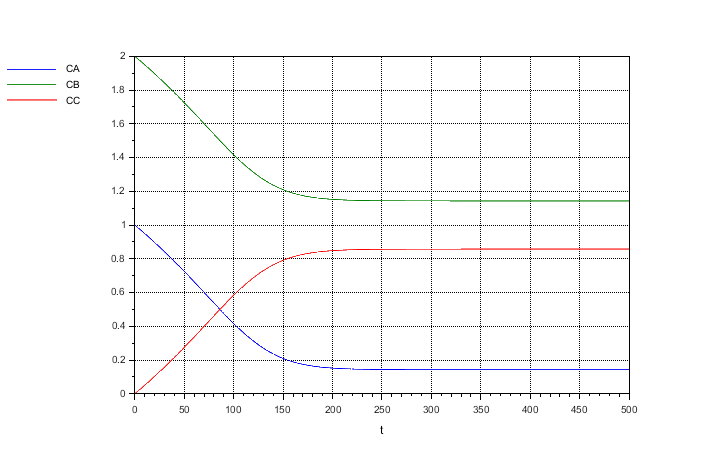
\includegraphics[width=0.6\textwidth]{Imagenes/RDMP_3.1C.png}
	\caption{Evolución de la conversión frente al tiempo en el reactor}
	\label{fig:RDMP-3.1C}
\end{figure}


\begin{figure}[h!]
	\centering
	\begin{subfigure}{0.48\textwidth}
		\centering
		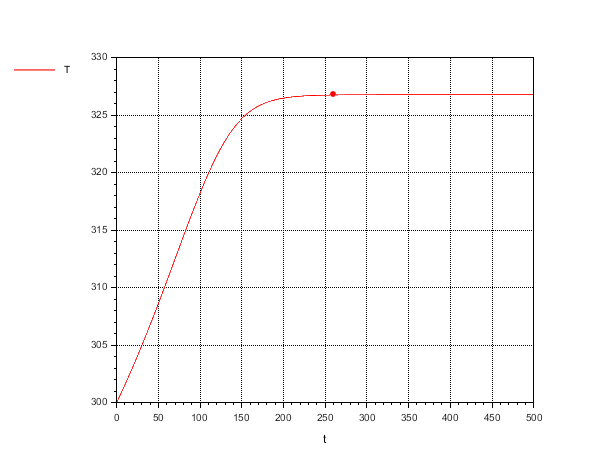
\includegraphics[width=\linewidth]{Imagenes/RDMP_3.2C.png}
		\caption{Temperatura frente tiempo}
		\label{fig:RDMP-3.2C}
	\end{subfigure}
	\hfill
	\begin{subfigure}{0.48\textwidth}
		\centering
		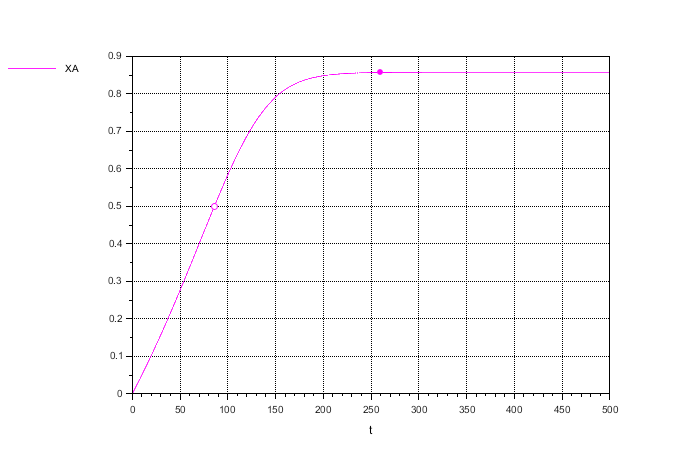
\includegraphics[width=\linewidth]{Imagenes/RDMP_3.3C.png}
		\caption{Conversión frente tiempo}
		\label{fig:RDMP-3.3C}
	\end{subfigure}
	\caption{Evolución de la conversión y temperatura en el reactor}
	\label{fig:RDMP-comparacion}
\end{figure}
\begin{figure}[h!]
	\centering
	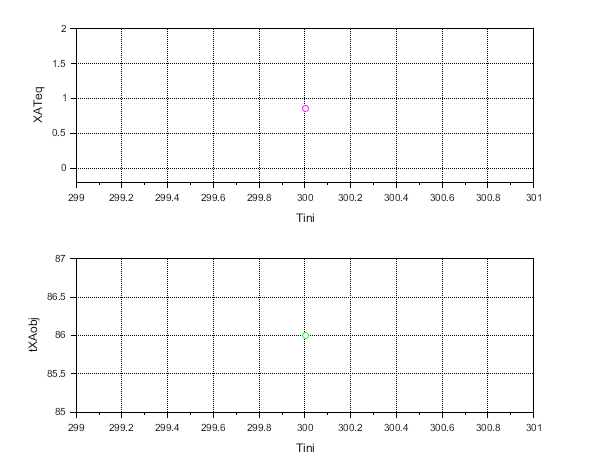
\includegraphics[width=0.6\textwidth]{Imagenes/RDMP_3.4C.png}
	\caption{Evolución de la conversión y temperatura en el reactor}
	\label{fig:RDMP-3.4C}
\end{figure}
\qs{RDMP-6}{En un reactor discontinuo mezcla perfecta se realiza el siguiente equilibrio químico durante 5 h a partir de 1 mol/L de A.
	A $\rightleftarrows$ B

	Factor preexponencial de Arrhenius directo = 1.94E15 h$^{-1}$\\
	Factor preexponencial de Arrhenius inverso = 6.26E19 h$^{-1}$\\
	Energía de activación directa = 44500 cal/mol\\
	Energía de activación inversa = 59500 cal/mol\\
	Temperatura máxima de operación = 650 K


	\begin{enumerate}[label=\bfseries\scriptsize\protect\circled{\footnotesize\Alph*}]
		\item Para una conversión dada, obtener la relación entre temperatura y velocidad de reacción
		\item Determinar la progresión óptima de temperatura
		\item Determinar la conversión máxima que se puede alcanzar siguiendo una progresión óptima de temperatura
	\end{enumerate}}
\nt{el ultimo es nuevo de este año sustituye los 2 anteriores}
\begin{minted}[fontsize=\small, linenos]{scilab}
clear; clc; 
// RDMP-6.sce
// A <=> B
// Progresión óptima de temperatura

// (a)

// CONSTANTES
kd0 = 1.94E15; ki0 = 6.26E19; // h-1
Ed = 44500; Ei = 59500; // cal/mol
R = 1.987; // cal/(mol*K)
Tmin = 500.0; dT = 0.1; Tmax = 650.0; T = Tmin:dT:Tmax; // K
kd = kd0*exp(-Ed./(R*T)); // Ecuación de Arrhenius directa
ki = ki0*exp(-Ei./(R*T)); // Ecuación de Arrhenius inversa

// CONDICIONES INICIALES
CAini = 1; CBini = 0; // mol/L

XA = 0.0;

CA = CAini - CAini*XA
CB = CBini + CAini*XA

// Velocidad de reacción
// r = rd - ri
r = kd*CA - ki*CB;
// Velocidad máxima
[rmax,indexTopt] = max(r)
// Temperatura óptima
Topt = T(indexTopt)

// GRÁFICAS
scf(1);  
plot(T,r,Topt,rmax,'bo');
xgrid; xlabel('T'); ylabel('r');
a1 = gca;
a1.log_flags = "nl" ;

// (b)

// SISTEMA DE ECUACIONES DIFERENCIALES
function dxdt = f(t,x)
    // Variables diferenciales
    CA = x(1)
    CB = x(2)
    // Velocidad de reacción
    // r = rd - ri
    r = kd*CA - ki*CB
    // Velocidad máxima
    [rmax,indexTopt] = max(r)
    // Temperatura óptima
    Topt = T(indexTopt)
    // Balance de materia para A
    // d(V*CA)dt = -rmax*V
    dCAdt = -rmax   
    // Balance de materia para B
    // d(V*CB)dt = rmax*V
    dCBdt =  rmax   
    // Derivadas
    dxdt(1) = dCAdt
    dxdt(2) = dCBdt
    dxdt(3) = Topt  // Almacenar Topt
endfunction

// CONDICIONES INICIALES
xini = [CAini; CBini; 0];

// TIEMPO
tfin = 5; dt = 0.01; t = 0:dt:tfin; // h

// RESOLVER
x = ode(xini,0,t,f);
CA = x(1,:); CAfin = CA($);
CB = x(2,:); CBfin = CB($);
Topt = diff(x(3,:))/dt; Toptfin = Topt($);
XA = 1 - CA/CAini; XAfin = XA($);
disp("La concentracion final de A es: " + string(CAfin) + " mol/L")
disp("La concentracion final de B es: " + string(CBfin) + " mol/L")
disp("La conversion final de A es: " + string(XAfin*100) + " %")
disp("La temperatura optima es: " + string(Toptfin) + " K")
// GRÁFICAS
scf(2); clf(2); 
plot(t,XA,'m-');
xgrid; xlabel('t'); legend('XA',-2,%f);

scf(3); clf(3); 
plot(t(1:$-1),Topt,'r-');
xgrid; xlabel('t'); legend('Topt',-2,%f);

indexTc = find(Topt<Tmax-1E-6,1);
tTc = t(indexTc)
Tc = Topt(indexTc)
disp("La temperatura de control es: " + string(Tc) + " K")
disp("El tiempo de control es: " + string(tTc) + " h")
plot(tTc,Tc,'ro');
 //! probar para diferentes conversiones el grafico 1 
\end{minted}
\nt{Revisar la linea de tTC y Tc ademas de revisar el ultimo comentario}
\Res{
	\begin{array}{l}
		\text{  La concentracion final de A es: 0.1573513 mol/L} \\
		\text{La concentracion final de B es: 0.8426487 mol/L}   \\
		\text{La conversion final de A es: 0.8426487}            \\
		\text{La temperatura optima es: 611.29273 K}             \\
		\text{La temperatura de control es: 649.85498 K}         \\
		\text{El tiempo de control es: 0.97 h}
	\end{array}
}
\begin{figure}[h!]
	\centering
	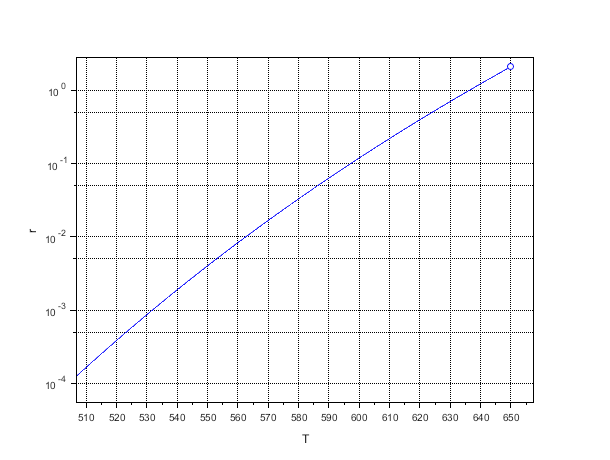
\includegraphics[width=0.5\textwidth]{Imagenes/RDMP_6.1.png}
	\caption{Velocidad de reacción frente a la temperatura}
	\label{fig:RDMP-6.1}
\end{figure}


\begin{figure}[h!]
	\centering
	\begin{subfigure}{0.48\textwidth}
		\centering
		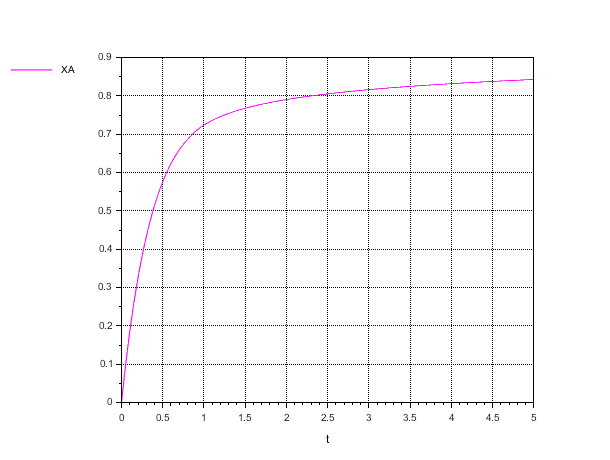
\includegraphics[width=\linewidth]{Imagenes/RDMP_6.2.png}
		\caption{Conversión frente tiempo}
		\label{fig:RDMP-6.2}
	\end{subfigure}
	\hfill
	\begin{subfigure}{0.48\textwidth}
		\centering
		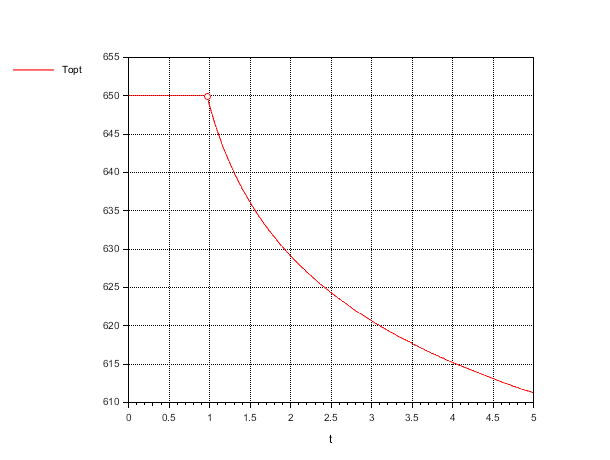
\includegraphics[width=\linewidth]{Imagenes/RDMP_6.3.png}
		\caption{Temperatura frente tiempo}
		\label{fig:RDMP-6.3}
	\end{subfigure}
	\label{fig:RDMP-6}
\end{figure}
\newpage
\qs{RDMP-MULT-1}{En un reactor discontinuo mezcla perfecta, se llevan a cabo las siguientes reacciones químicas:

	A $\rightarrow$ B  , k$_1$ = 0.01 min$^{-1}$\\
	B $\rightarrow$ C  , k$_2$ = 0.01 min$^{-1}$\\
	C $\rightarrow$ B  , k$_3$ = 0.05 min$^{-1}$\\
	B $\rightarrow$ D  , k$_4$ = 0.02 min$^{-1}$

	\begin{enumerate}[label=\bfseries\scriptsize\protect\circled{\footnotesize\Alph*}]
		\item Obtener la dinámica de 500 min si la reacción se pone en marcha con 1 mol/L del compuesto A
		\item Determinar durante cuánto tiempo:
		      \begin{itemize}
			      \item La concentración de A es mayor a 0.5 mol/L
			      \item La concentración de B está entre 0.15 y 0.20 mol/L
			      \item La concentración de C crece
			      \item La concentración de D es predomina
		      \end{itemize}
	\end{enumerate}}

\begin{minted}[fontsize=\small, linenos]{scilab}
  clear; clc; 
// RDMP-MULT-1.sce
// 1) A => B
// 2) B => C
// 3) C => B
// 4) B => D
// Isotermo

// SISTEMA DE ECUACIONES DIFERENCIALES
function dxdt = f(t,x)
    // Variables diferenciales
    CA = x(1)
    CB = x(2)
    CC = x(3)
    CD = x(4)
    // Velocidades de reacción
    r1 = k1*CA
    r2 = k2*CB
    r3 = k3*CC
    r4 = k4*CB
    // Balance de materia para A
    // d(V*CA)dt = -r1*V
    dCAdt = -r1
    // Balance de materia para B
    // d(V*CB)dt = (r1-r2+r3-r4)*V
    dCBdt = r1-r2+r3-r4
    // Balance de materia para C
    // d(V*CC)dt = (r2-r3)*V
    dCCdt = r2-r3
    // Balance de materia para D
    // d(V*CD)dt = r4*V
    dCDdt = r4
    // Derivadas
    dxdt(1) = dCAdt
    dxdt(2) = dCBdt 
    dxdt(3) = dCCdt
    dxdt(4) = dCDdt
endfunction

// CONSTANTES
k1 = 0.01; k2 = 0.01; k3 = 0.05; k4 = 0.02; //min-1

// CONDICIONES INICIALES
CAini = 1; CBini = 0; CCini = 0; CDini = 0; // mol/L
xini = [CAini;CBini;CCini;CDini];

// TIEMPO
tfin = 500; dt = 0.1; t = 0:dt:tfin; //min

// RESOLVER
x = ode(xini,0,t,f);

CA = x(1,:); CAfin = CA($)
CB = x(2,:); CBfin = CB($)
CC = x(3,:); CCfin = CC($) 
CD = x(4,:); CDfin = CD($) 

// GRÁFICAS
scf(1); clf(1); 
plot(t,CA,t,CB,t,CC,t,CD);
xgrid; xlabel('t'); legend('CA','CB','CC','CD',-2,%f);

CAobj = 0.5;
indexA = find(CA > CAobj);
tA = dt*length(indexA)
disp('tiempo para CA = 0.5 mol/L ='+string(tA)+'min');
plot(t(indexA),CA(indexA),'b.');

CBlo = 0.15; CBup = 0.20;
indexB = find(CB > CBlo & CB < CBup);
tB = dt*length(indexB)
disp('tiempo para 0.15 < CB < 0.20 mol/L ='+string(tB)+'min');
plot(t(indexB),CB(indexB),'g.');

dCCdt = diff(CC)/dt;
indexC = find(dCCdt > 0);
tC = dt*length(indexC);
disp('tiempo para dCCdt > 0 ='+string(tC)+'min');
plot(t(indexC),CC(indexC),'r.');

indexD = find(CD == max(CA,CB,CC,CD));
tD = dt*length(indexD);

plot(t(indexD),CD(indexD),'c.');
disp('tiempo para CD máximo ='+string(tD)+'min');
indextD = find(CD > CA ,1);
disp('tiempo para CD > CA ='+string(t(indextD))+'min');
\end{minted}
\begin{figure}[h!]
	\centering
	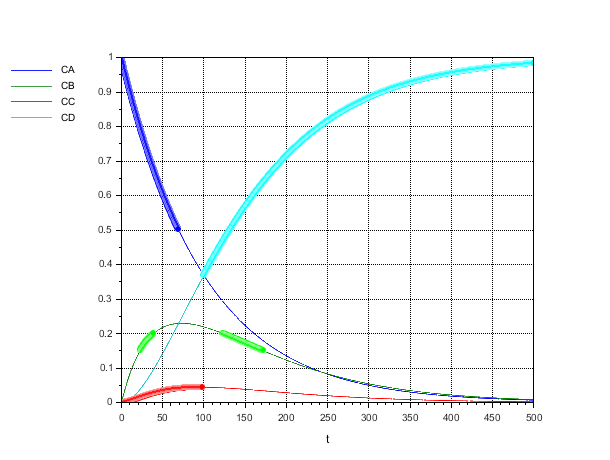
\includegraphics[width=0.5\textwidth]{Imagenes/RDMP_Multi_1.png}
	\caption{Evolución de la concentración frente al tiempo en el reactor}
	\label{fig:RDMP-MULT-1}
\end{figure}
\Res{
	\begin{array}{l}
		\text{tiempo para CA = }0.5 \text{ mol/L =}69.4\text{min} \\
		\text{tiempo para 0.15 < CB < 0.20 mol/L =}65.8\text{min} \\
		\text{tiempo para dCCdt > 0 =}98.4\text{min}              \\
		\text{tiempo para CD máximo =}400.2\text{min}             \\
		\text{tiempo para CD > CA =}99.9\text{min}
	\end{array}
}
\newpage

\qs{RDMP-MULT-2}{Un reactor discontinuo mezcla perfecta de 1 m$^3$ se pone en marcha a 303 K con 1 mol/L del compuesto A,
	transcurriendo las siguientes reacciones químicas en disolución acuosa sin generación apreciable de calor durante 2 h:

	A $\rightarrow$ B  , k$_1$ = exp(-1500/T +\hspace{0.5\baselineskip}  6) h$^{-1}$\\
	A $\rightarrow$ C  , k$_2$ = exp(-4000/T + 12) h$^{-1}$\\
	B $\rightarrow$ D  , k$_3$ = exp(-3000/T + 10) h$^{-1}$

	\begin{enumerate}[label=\bfseries\scriptsize\protect\circled{\footnotesize\Alph*}]
		\item Considerando que D es el compuesto deseado, determinar cómo debe operar la camisa
	\end{enumerate}}
\begin{minted}[fontsize=\small, linenos]{scilab}
  clear; clc; 
// RDMP-MULT-2.sce
// 1) A => B
// 2) A => C
// 3) B => D*
// No adiabático

// SISTEMA DE ECUACIONES DIFERENCIALES
function dxdt = f(t,x)
    // Variables diferenciales
    CA = x(1)
    CB = x(2)
    CC = x(3)
    CD = x(4)
    T  = x(5)
    // Ecuaciones de Arrhenius
    k1 = exp(-1500/T +  6); //h-1
    k2 = exp(-4000/T + 12); //h-1
    k3 = exp(-3000/T + 10); //h-1
    // Velocidades de reacción    
    r1 = k1*CA
    r2 = k2*CA
    r3 = k3*CB
    // Balance de materia para A
    // d(V*CA)dt = (-r1-r2)*V
    dCAdt = -r1 - r2
    // Balance de materia para B
    // d(V*CB)dt = (r1-r3)*V
    dCBdt =  r1 - r3
    // Balance de materia para C
    // d(V*CC)dt = r2*V
    dCCdt =  r2
    // Balance de materia para D
    // d(V*CD)dt = r3*V
    dCDdt =  r3
    // Temperatura de la camisa
    if t < tfin/2 then TJ = TJ1;
        else TJ = TJ2;
    end
    // Calor transferido del reactor a la camisa
    Q = U*A*(TJ-T)
    // Balance de energía 
    // d(V*RHO*CP*T) = Q
    dTdt = Q/(V*RHO*CP) 
    // Derivadas
    dxdt(1) = dCAdt
    dxdt(2) = dCBdt
    dxdt(3) = dCCdt
    dxdt(4) = dCDdt
    dxdt(5) = dTdt
endfunction

// CONSTANTES
V = 1; // m3
A = 5; // m2
U = 1000; // kcal/(h*m2*K)
RHO = 1000; // kg/m3
CP = 1; // kcal/(kg*K)
Tcold = 293; Thot = 353; // K 

// Operación de la camisa
//! Esta para una operacion en exclusiva la del caso 1 probar a meter en un bucle for para encontrar la maxima 
op =1;
select op
    case 1 then TJ1 = Tcold; TJ2 = Tcold; // K
    case 2 then TJ1 = Thot;  TJ2 = Thot;  // K
    case 3 then TJ1 = Tcold; TJ2 = Thot;  // K
    case 4 then TJ1 = Thot;  TJ2 = Tcold; // K
end

// CONDICIONES INICIALES
CAini = 1; CBini = 0; CCini = 0; CDini = 0; // mol/L
Tini = 303; //K
xini = [CAini; CBini; CCini; CDini; Tini];

// TIEMPO
tfin = 2; dt = 0.01; t = 0:dt:tfin; //h

// RESOLVER
x = ode(xini,0,t,f);
CA = x(1,:); CAfin = CA($);
CB = x(2,:); CBfin = CB($);
CC = x(3,:); CCfin = CC($);
CD = x(4,:); CDfin = CD($);
T  = x(5,:); Tfin = T($);
disp('CAfin ' + string(CAfin) + ' mol/L');
disp('CBfin ' + string(CBfin) + ' mol/L');
disp('CCfin ' + string(CCfin) + ' mol/L');
disp('CDfin ' + string(CDfin) + ' mol/L');
disp('Tfin ' + string(Tfin) + ' K');

// GRÁFICAS
scf(1);clf(1);
plot(t,CA,t,CB,t,CC,t,CD);
xgrid; xlabel('t'); legend('CA','CB','CC','CD',-2,%f);

scf(2);clf(2);
plot(t,T);
xgrid; xlabel('t'); legend('T',-2,%f);

scf(3);
bar(op,[CAfin,CBfin,CCfin,CDfin],'stacked');
xgrid; xlabel('op'); legend('CA','CB','CC','CD',-2,%f);


//* Probar a hacer graficas para las concentraciones a diferentes T con el bucle for dentro 
\end{minted}
\begin{figure}[h!]
	\centering
	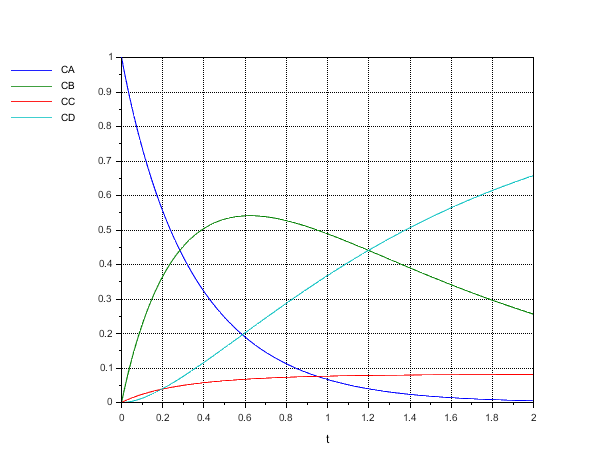
\includegraphics[width=0.65\textwidth]{Imagenes/RDMP_Multi_2.1.png}
	\caption{Evolución de la concentración frente al tiempo en el reactor}
	\label{fig:RDMP-MULT-2.1}
\end{figure}
\begin{figure}[h!]
	\centering
	\begin{subfigure}{0.48\textwidth}
		\centering
		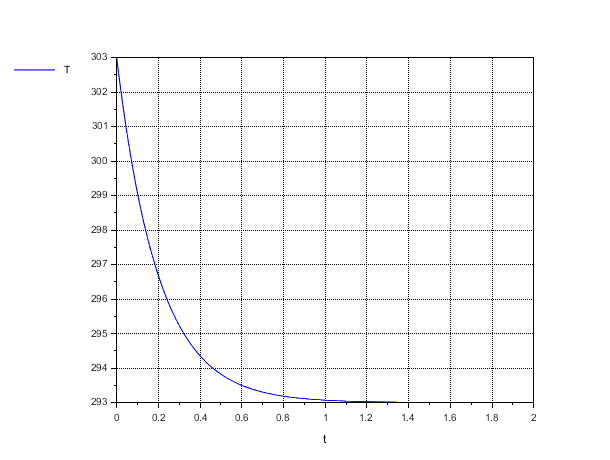
\includegraphics[width=\linewidth]{Imagenes/RDMP_Multi_2.2.png}
		\caption{Evolución de la Temperatura frente al tiempo en el reactor}
		\label{fig:RDMP-MULT-2.2}
	\end{subfigure}
	\hfill
	\begin{subfigure}{0.48\textwidth}
		\centering
		\includegraphics[width=\linewidth]{Imagenes/RDMP_Multi_2.3.png}
		\caption{Concentraciones finales en funcion de la operacion de la camisa}
		\label{fig:RDMP-MULT-2.3}
	\end{subfigure}
\end{figure}
\Res{
	\begin{array}{l}
		\text{CAfin } 0.0049216 \text{ mol/L} \\
		\text{CBfin } 0.2559964 \text{ mol/L} \\
		\text{CCfin } 0.0810131 \text{ mol/L} \\
		\text{CDfin } 0.658069 \text{ mol/L}  \\
		\text{Tfin } 293.00045 \text{ K}
	\end{array}
}

\end{document}
